Outlier detection is concerned with detecting outliers in data. Hawkins defines outliers as ``an object that deviates so much from the rest of the data as to arouse suspicion that it was generated by a different mechanism''. Outliers are different from noise. Noise is random error or variance in a measured variable. Outliers are interesting, because they violate the mechanism that generates normal data.

There are different types of outliers
\begin{itemize}
    \item \textbf{Global outliers:} Objects that significantly deviate from the data set
    \item \textbf{Contextual outliers:} Object that deviates based on context, such as temperature in a given city (may make sense somewhere else, but context says it may be an outlier). Here contextual attributes define context and behavioral attributes define the characteristics, which is what is used in outlier evaluation
    \item \textbf{Collective outliers:} Whole sets of object may collectively constitute an outlier. For example a number of suspicious network packets
\end{itemize}

Challenges of outlier detection are 

\begin{itemize}
    \item Modelling the normal objects and outliers properly. It is difficult to enumerate all possible normal behaviors. The difference between normal and outlier objects is often a gray area
    \item Application-specific outlier detection. What is an outlier may be applciation dependant.
    \item Understandability. This could be something like specifying to which degree something is an outlier
\end{itemize}

Some different outlier methods are 
\begin{itemize}
    \item \textbf{Supervised methods:} Are useful if one can contain user-labeled examples of outliers. Then we can consider outlier detection a classification problem. The challenges here are imbalanced classes (outliers rare in the data set). 
    \item \textbf{Unsupervised methods:} This cannot detect collective outliers effectively. Normal objects may not share strong patterns, but collective outliers may share high similarity. Can also use clustering, first we need clusters, then outliers. This can make it hard to distinguish noise from outliers, and is costly.
    \item \textbf{Semi-supervised methods:} We may labels on some of our data, some of them outliers, some of them not. Here the problem is one of semi-supervised learning.
    \item \textbf{Statistical approaches:} This assumes an underlying model that can generate the dataset. For example, if the data is normally distributed, we can look at the probability of a certain point. Typically we look at $3$ times standard deviation. Most tests are for single attributes only, and the distribution may not be known. Statistical tests are sensitive to outliers.
\end{itemize}

\subsection{Model based methods}
    \emph{Model-based} statistical methods assume that the data follows a distribution. Then it uses this to find outliers. 
    
    Effectiveness highly depends on if the assumption holds for real data. There are a number of approaches that we can use, such as parametric and non-parametric models. 
    
    We can also use \emph{parametric and mixed models}. For example, we an use several parametric distributions to fit the data, such as two normal distributions. The probability that $o$ is generated by a mixture of two Gaussians is
    \m{
        P(o | \theta_1, \theta_2) = f_{\theta_1}(o) + f_{\theta_2}(o)
    }
    Where $f_\theta$ are the PDFs. We can use the EM algorithm to learn the parameters $(\mu_i, \theta_i)$. 
    
    An example of non-parametric models is the Histogram. Here the model is learned from the input data without any a-priori assumptions. The problem with a Histogram for example, is that it is difficult to choose an appropriate bin size. Too small and you get rare and emptuy bins, too big and the outliers are in non-outlier bins. A solution to this is \emph{kernel density estimation} to estimate the PDF. If high, objects are normal, otherwise they are likely an outlier.
    

\subsection{Depth-based approaches}
    The idea behind depth-based approaches is to look for outliers at the boundaries of the data space. For example we could create layers of Convex Hulls in the data space. The outliers are then objects on the boundaries of the outlier layers. 
    
    This assumes that outliers are located at the border of the data space, and that normal objects are located in the center of the data space. 
    
    We can also say that all objects which depth is smaller than some $k$ are outliers.
    
    \begin{center}[h]
        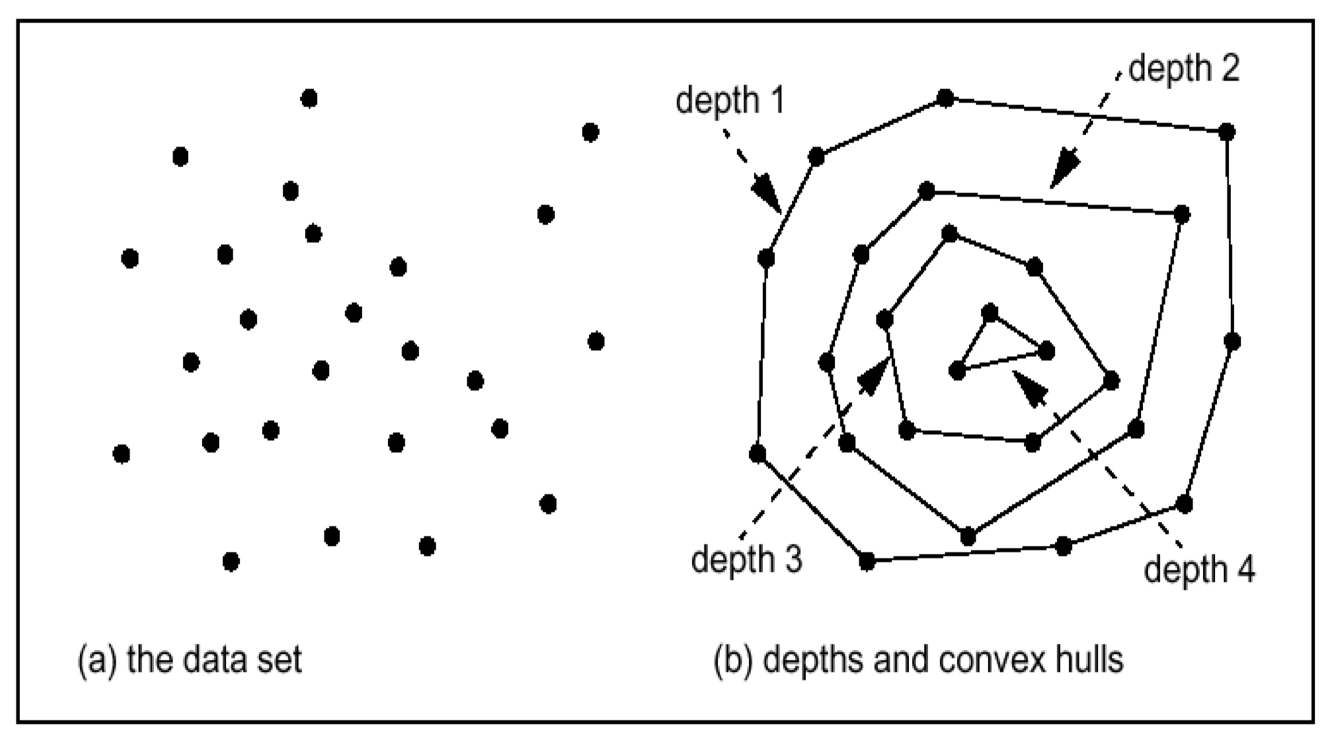
\includegraphics[width=0.5\textwidth]{images/layers.png}
    \end{center}
    
    The advantages of depth-based approaches is 
    \begin{itemize}
        \item Uses a global reference set for outlier detection
        \item Originally outputs a label, but can be extended for scoring easily, take depth as a scoring value for example
    \end{itemize}
    
    The disadvantages are
    \begin{itemize}
        \item Convex hull computation is usually only efficient in 2D and 3D spaces
    \end{itemize}
    
\subsection{Proximity and distance based models}
    Proximity and distance based models try to overcome the limitations of statistical models. It performs multi-dimensional analysis without knowing the distribution of the data.
    
    An example of a heuristic is that an object is an outlier of its nearest neighbour is far away. For example, this distance significantly deviates from other objects distance in this regard. 
    
    \textbf{DB($\varepsilon, \pi$)-outliers} works as follows:
    \begin{itemize}
        \item Given a radius $\varepsilon$ and a percentage $\pi$
        \item A point is considered an outlier if at most $\pi$ percent of all other points have a distance to $p$ less than $\varepsilon$
        \item The outliers are $\set{
            p | \frac{
            |\set{q \in D | dist(p,q) \lt \varepsilon}|}{|D|}
            \leq \pi}$
    \end{itemize}
    In plain English, if too small a fraction has a small distance to $p$, then a high fraction must have a large distance to it, making it an outlier. 
    
    There are limitations to DB-outliers.
    For $o_1$ we have that it is a clear outlier for $\pi \geq 0.99$ and a large $\varepsilon$. $o_2$ is not very well captured, because either it is not an outlier, or many points in $C_1$ are definitely also outliers. It therefore only captures global outliers. Objects that are outlying relative to their locl neighbour are also deviating.
    
    \begin{center}[h]
        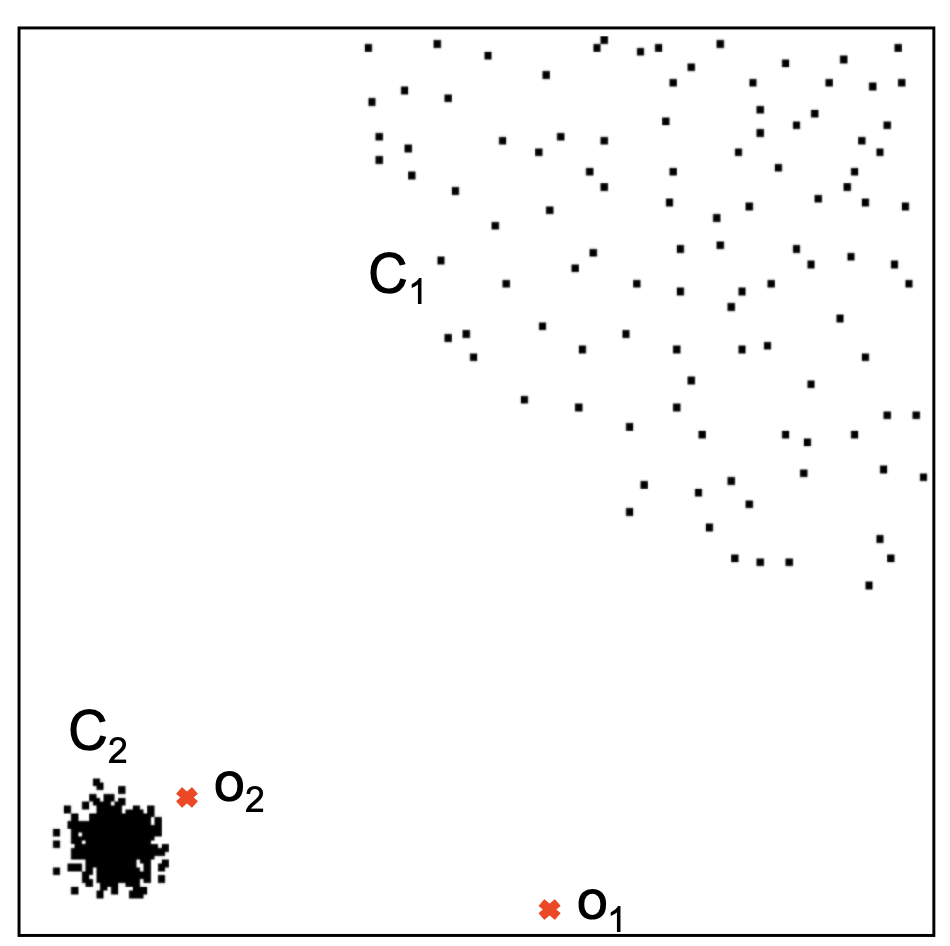
\includegraphics[width=0.2\textwidth]{images/DBOUTLIERS.png}
    \end{center}
    
    The advantages of proximity-based methods is that they are easy to implement, they give a global view, but require parameterisation. The disadvantages are that the effectiveness of proximity-based methods is highly reliant on the measure. It cannot easily detect groups of outliers, and requires tuning of parameters.
    
\subsection{Density-based methods}
    The idea behind density-based methods is to compare the density around a point with the density around its local neighbours. The relative density of a point compared to its neighbours is computed as an outlier score. Approaches also differ in how to estimate density.
    
    The basic assumption is that the density around a normal object is to similar to the density around its neighbours. The density around an outlier is considerably different to the density around its neighbours. 
    Instead of looking for global outliers, we look for global outliers. The basic idea is as follows: Look at the $k$-nearest neighbour distance of $p$ relative to the $k$-nearest neighbor distances of these $k$ neighbours relative to $p$. This finds local outliers. Each object has an outlier factor, which is the degree to which it deviates. 
    
    We need the following concepts for density-based clustering
    
    \begin{itemize}
        \item \textbf{$k$-nearest neighbour distance:} Distance between $o$ and its $k$-nearest neighbour. 
        \item \textbf{Reachability distance:} Introduces a smoothing factor. \m{
        reach_dist_k(p, o) = \max\set{kdist(o), dist(p, o)}
        }
        \item \textbf{Local reachability distance (lrd) of $p$:} Inverse of the average reachdists of the kNNs $(N_k(p))$ of $p$ \m{
        lrd_k(p) = \frac{
            \frac{1}{\sum_{o \in N_k(p){reachdist_k(p, o)}}}
        }{|N_k(p)|}
        }
        \item \textbf{Local outlier factor (LOF) of point $p$:} Average ratio of lrds of neighbors of $p$ and lrd of $p$ \m{
            LOF_k(p) = 
            \frac{
                \sum_{o \in N_k(p)\frac{lrd_k(o)}{lrd_k(p)}}
            }{|N_k(p)|}}
    \end{itemize}
    LOF is big if LRD of neighbours is big. This implies that neighbours are in denser regions than $p$. 
    
\subsection{Clustering-based methods}
    A cluster is a maximal set of density-connected objects, separated by sparsely populated areas in feature space. Therefore, every object not contained in a cluster must be an outlier. 
    
    This uses the concept of complementarity, which is that we get the same result per object of clustering and outlier detection.

    We can for example use DBSCAN noise as outliers. We can also use $k$-means to partition data points into clusters. Then for each object $o$, we assign an outlier score based on its closest center. If $dist(o, c_o)/avgdist(c_o)$ is large, then it is likely an outlier. 
    
\subsubsection{FindCBLOF}
    FindCBLOF detects outliers in small clusters. We find the clusters, sort them in decreasing size. We assign a cluster-based local outlier factor to each point (Hence the CBLOF).
    
    \begin{itemize}
        \item If objet $p$ belongs to a large cluster $C_i$, then $CBLOF(p) = |C_i| \cdot S$, $S$ is similarity between $p$ and the cluster
        \item If $p$ belongs to a small cluster, then $CBLOF(p) = |C_i| \cdot S$ where $S$ is the similarity between $p$ and the closest large cluster.
    \end{itemize}
    
    It is possible to hit complementarity issues. Examples of non-complementary:
    \begin{itemize}
        \item $A$: Set of objects in line patterns
        \item $B$: Set of all objects in the disk pattern
        \item $o$ Object outside of $B$
    \end{itemize}
    DBScan is not able to detect $o$ as an outlier, and all objects in $A$ and $B$ as inliers. 
    
    \begin{center}
        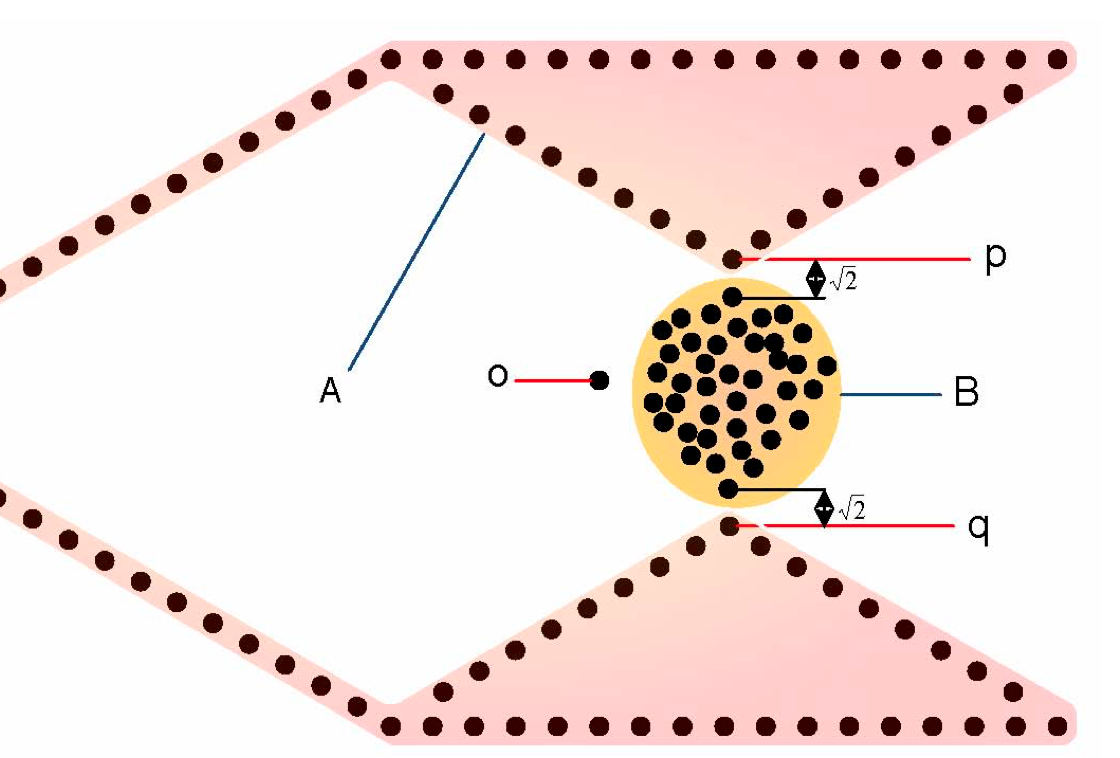
\includegraphics[width=0.5\textwidth]{images/noncomplement.png}
    \end{center}
    
    The advantages of clustering based methods is
    \begin{itemize}
        \item It can detect without requiring labels
        \item Works for many types of data
        \item Clusters can be regarded as summaries of the data
        \item Once we have our clusters, we need only compare any object against the clusters in order to see if its an outlier
    \end{itemize}
    The disadvantages are
    \begin{itemize}
        \item The effectiveness depends on the clustering method uses. They may not be optimized for the purpose
        \item There is high computational cost because we need to find the clusters first
    \end{itemize}
    
\subsection{Outlier detection in high-dimensional data}
    There are a number of challenges with high-dimensional data. The curse of dimensionality means that the contrast between distances decreases as the dimensions increase. Additionally, in high-dimensional space, data is sparse, which makes for more outliers. The concept of neighbours also becomes meaningless.
    
    There is also the problem of scalability. The number of subspaces increases exponentially with the number of dimensions. 
    
    The solution is to use more robust distance functions and find full-dimensional outliers. For example, by using projections.
    
\subsubsection{HilOut}
    the idea behind the HilOut algorithm is to find distance-based outliers, but to use ranks of distance instead of the absolute distance. 
    
    For each object $o$, we find the $k$-nearest neighbours $nn_1(o), \dots, nn_k(o)$. The weight of each object $o$ is then $w(o) = \sum_{i=1}^{k}{dist(o, nn_i(o))}$.
    
    All objects are then ranked in weight-descending order. Top-$l$ objects in weight are output as outliers. 
    
\subsubsection{Finding outliers in subspaces}
    Finding outliers in much lower dimensional subspaces is easier to interpret. 
    
    For example, we could use a grid-based subspace outlier detection method. We project data onto various subspaces to find an area whose density is much lower than average. 
    
    We discretize the data into a grid with $\phi$ equi-depth (same number of points) regions. 
    \begin{itemize}
        \item Consider a $k$d cube $C$. $k$ ranges on $k$ dimensions with $n$ objects. 
        \item If attributes are independently distributed, then let $f = \frac{1}{\phi}$. The expected number of objects in that $k$-dimensional region is $(\frac{1}{\phi})^2n = f^kn$. Think of a Bernoulli variable where there is some probability that it lands in that grid. The standard deviation is $\sqrt{f^k(1-f^k)n}$
        \item The sparsity coefficient of a cube $C$ is \m{
            S(C) = \frac{n(C) - f^k n}{\sqrt{f^k (1-f^k) n}}
        }
        \item If $S(C) < 0$, then $C$ contains fewer objects $n(C)$ than expected
        \item The more negative it is, the sparse $C$ is, and the more likely that objects in $C$ are outliers in the subspace.
    \end{itemize}

\subsection{Angle-based outlier detection (ABOD)}
    In high-dimensional data, angles are more stable than distances. An object is considered an outlier if most other objects are located in similar directions, and an inliner if many other objects are located in varying directions.
    
    \begin{center}
        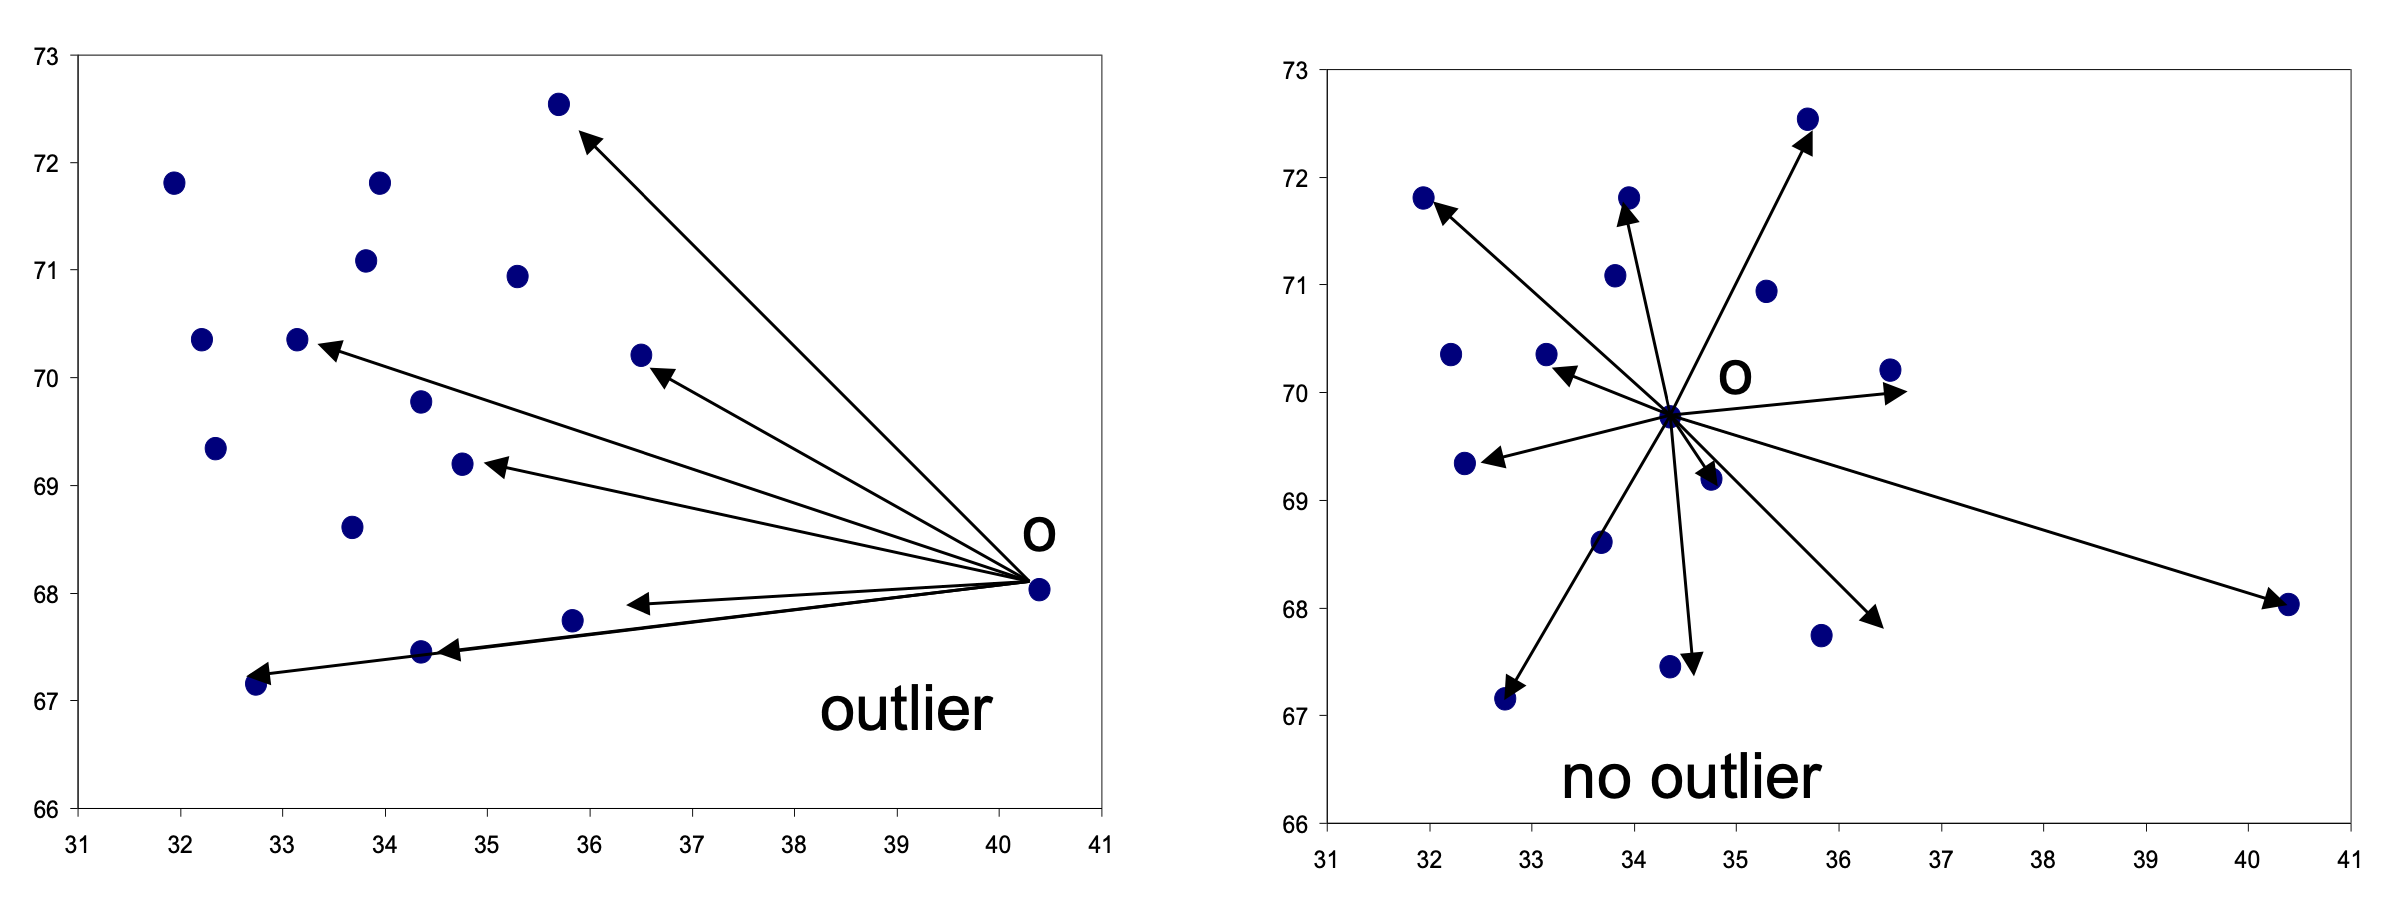
\includegraphics[width=1\textwidth]{images/angles.png}
    \end{center}
    
    The basic assumption behind the ABOD is that outliers are at the borders of the data distribution, and that normal points are in the center.
    
    The model is as follows:
    \begin{itemize}
        \item Consider the angle for a point $p$ between $p_x, p_y$ for any two points in our DB
        \item Consider the spectrum of all these angles
        \item The broadness of the spectrum is a score for the outlierness of a point
    \end{itemize}
    
    We can measure the variance of the angle spectrum. Weighted by the corresponding distances (for lower dimensional data sets where angles are less reliable). We can then compute an ABOD score
    
    \m{
        ABOD(p) = VAR_{x, y \in DB}(\frac{
        \langle x -p, y-p \rangle}{||x-p||^2 \cdot ||y-p||^2})
    }
    Here a small ABOD means that it is an outlier, and a high ABOD means that it is not an outlier. 
    
    There are some ideas for ABOD algorithms: Naive ABOD algorithms take $O(n^3)$. It is an approximate algorithm based on random sampling for mining the top $n$ outliers. We do not consider all pairs of other points $x, y$ in the DB to compute the angles. We compute ABOD based on samples to get a lower bound of the real ABOD. We filter out points that have a high lower bound. We then refine (compute exact value of ABOD) only for a small number of points
    
    This is a global approach to outlier detection and outputs an outlier score.
    
    
\subsection{HiCS: High contrast subspaces}
    The idea behind HiCS is to find subspaces with high contrast that could potentially reveal outliers. 
    
    Step $1$ would be to find uncorrelated subspaces. The PDF of a value in a 1D projection is the same as the conditional PDF of that value given the values in other dimensions. We want to find subspaces with unexpected non-uniformity, which is more likely to contain outliers. 
    
    Step $2$ would be to perform the actual outlier detection. We can run LOF on these subspaces to find outliers, aggregate scores from multiple subspaces to obtain robust results. We can then use something like statistical tests to assess our subspaces.
    
    Marginal densities are 1d projections that are independent of any subspace.
    
    Non-uniformity testing works as follows:
    \begin{enumerate}
        \item Generate random rectangular region of dimension $p$. The width of random range along each dimension is selected such that 1d range contains $N \cdot \alpha^{\frac{1}{p}}$ points, where $\alpha < 1$. This implies that the $p$-dimensional region is expected to contain $N \alpha$ points. We then test the dimensions. $i$th dimension is used for hypothesis testing, where the dimension $i$ is chosen at random
        \item Set of points $s_i$ in intersection of ranges remaining in $(p-1)$ dimensions. 
        \item Fraction within upper bound and lower bounds of range of dimension $i$ is an estimate of the conditional probability of the value in $i$ given other dimensions
        \item The deviation of $s_i$ w.r.t to expecation is determined using statistical hypothesis testing
    \end{enumerate}
    Repeat multiple times over different random ranges and test dimensions. Average the deviation values over multiple tests. The subspaces with large deviations are those with high contrast.
    
    Finally, remove redundant subspace of dimension $p$ if subspace of dimension $p+1$ has higher contrast.
    
    The conditional PDF of attribute $s_i$ is defined by conditioning over all other attributes \m{
        p_{s_i | s \in S \backslash s_i}(x_{s_i | \set{x_s : s \in S \backslash s_i}})
    }
    Subspace contrast measure for subspace $S$ uses deviation measure between $\hat{p}_s$ (the marginal density of $s$ w.r.t to full data set) and $\hat{p}_{s | C}$ (density of $x_s$ w.r.t to remaining set that fulfills condition $C$).
    \m{
        contrast(S) = \frac{1}{M}\sum_{i}^{M}deviation(\hat{p}_s, \hat{p}_{s | C_i})
    }
    
    We can use the \emph{Welch t-test} in order to measure deviation. It is one of the statistical tests that we can use. 
    \begin{itemize}
        \item Consider sample means and estimated variances
        \item $t$ has a small value if both samples are from the same distribution (similar sample moments) \m{
            t = \frac{
            \hat{\mu}_{si} - \hat{\mu_i}_{s_i}'
            }{
            \sqrt{
                \frac{\hat{\sigma}_{s_i}^2 }{N} + \frac{\hat{\sigma}_{s_i}'^2}{N'}
            }
            }
        }
    \item This could be used directly, but here turned into probability by integration of the $t$ distribution
    \item $p_t$ is the probability of observing a larger absolute value than $t$ by chance if null hypothesis is fulfilled (same distribution). Deviation is then defined as $1 - p_t$
    \end{itemize}
    
    There is also the Kolmogorov-Smirnov test. it operates on data samples instead of moments. Deviation is defined as maximum difference between the two empircal CDFs $F_A$ for sample $A$ and $B$.
    \m{
        Deviation(\hat{p}_A, \hat{p}_B) = \sup_{x_{s_i}} | F_A(x_{s_i}) - F_B(x_i)|
    }
    Where $F$ is the percentage of objects whose value is less than some value
    \m{
        F(x_{s_i}) = \frac{1}{N}\sum_{y \in D} I[y_{s_i} < x_{s_i}]
    }

    The HiCS algorithm works bottom-up, just like for subspace clustering. From $d$-dimensional subspaces with contrast above threshold, we generate $(d+1)$-dimensional subspace candidates. It starts with two-dimensional instead of one-dimensional subspaces. There is no contrast (no sense of correlation) with 1D subspaces.
    
    We have no monotonicity property, but typically correlation in for example 3D is also reflected in 2D.
    
    The HiCS algorithm is then
    \begin{itemize}
        \item The parameters are $S, M, \alpha$
        \item It outputs the contrast of $S$
        \item For $i = 1 \dots M$
        \begin{itemize}
            \item Permute list of subspace attributes $s \in S$
            \item Initialise boolean vector selected\_objects for all objects to $T$
            \item For $i$ to $|S| - 1$:
            \item \begin{itemize}
                \item Select random index block of attribute $s_i$ with size of $N \cdot \sqrt[|S|]{\alpha}$
                \item Mask index block with selected\_objects
            \end{itemize}
            \item Compare distributions $deviation(\hat{p}_{s_i}, \hat{p}_{s_i | selected\_objects})$ for the remaining attribute with $i = |S|$
        \end{itemize}
        \item Combine results of all statistical tests
    \end{itemize}
    
    Note that it generates synthetic data. \footnote{elaborate}
    
    We then apply an outlier approach to subspaces with contrast, for example LOF. We can then aggregate results with methods such as averages and maxima. Average can mean that several outlying subspaces accumulate. Final output are scores which is used to produce ranking.
    
    The advantages of HiCS are
    \begin{itemize}
        \item It decouples subspace search and outlier detection
        \item statistical testing assumes correlation important for outliers. It is expected to work better for approaches such as LOF than other non-density based notions
        \item Other subspace outlier techniques are restricted to axis-parallel subspaces, which is not the case here
        \item Generated data also used for other studies both for outlier detection and subspace clustering
    \end{itemize}
    The disadvantages are that
    \begin{itemize}
        \item Might miss subspaces as it evaluates one with respect to others
        \item Based on randomization
        \item Potentially require enumeration of a large number of subspaces
    \end{itemize}
    
    
\subsection{Isolation Forests}
    We can also use decision trees to detect outliers. An outlier might be in a completely different part of a decision tree. Outliers generally have path lengths in decision trees that are small. 
    
    The isolation forest algorithm goes as follows:
    \begin{itemize}
        \item Randomly sample a subset of the data
        \item Build a tree from random sample
            \begin{itemize}
                \item Each tree is generated by randomly choosing a splitting atrribute and tree split point
                \item Tree is grown either until maxdepth is reached, only $1$ point remains or all attributes have the same values
            \end{itemize}
        \item Select the split feature $A$ uniformly random
        \item Select the split value $V_A$ uniformly as $\min(A) + (\max(A) - \min(A)) \cdot random(0, 1)$
        \item Grow random tree until each data point in its own leaf or tree reaches max height
    \end{itemize}
    
    Finally, to score a data point, we find the height of the leaf node. The smaller the height, the more anomalous is the point. 
    
    Build an ensemble of decision trees from randomly selected subsamples of size $n$. Use average expected height to compute the anomaly score. 0 is normality. $1$ is abnormality. 
    
    Basic notions of the score is
    \begin{itemize}
        \item Ensemble average path length $E(h(x))$ to point $x$
        \item Normalize by expected path length $c(n)$ of balanced binary search tree with $n$ data points. 
    \end{itemize}
    \m{
        s(x, n) = 2^{-\frac{E(h(x))}{c(n)}}
    }
    
\subsubsection{iTree algorithm}
    The iTree algorithm samples $S$ randomly drawn from $X \subseteq \R^d$. It takes parameters $S, l, l_\max$. 
    
    \begin{itemize}
        \item If $l \geq l_\max$ or $|S| \leq 1$ then return $exNode(S)$ and end
        \item else randomly select dimension $q \in \set{1, \dots, n}$
        \item Randomly select a split value $p$ between max and min values along dimension $q$ in $S$
        \item $S_l = filter(s, q \lt p$
        \item $S_r = filter(S, q \geq p$
        \item return $inNode(left = iTree(s_l, l + 1, l_\max), right = iTree(S_r, l + 1, l_\max),
        splitDim = q,
        splitVal = p
        )$
    \end{itemize}
    
    The advantages of iTree is
    \begin{itemize}
        \item Easy to construct (no distance or density function required) avoiding difficult decisions on if data points are anomalies or not
        \item Can achieve sublinear time complexity and a small memory footprint by exploiting subsampling. By eliminating major computational cost of distance calculation in all the distance and density based AD methods
        \item Can provide anomaly explanations
    \end{itemize}
    The disadvantages are
    \begin{itemize}
        \item hyperparameter tuning require,d such as number of trees, sample size and heights of trees
        \item Requires a high percentage of relevant features to identify anomalies. In presence of features do that not provide information over the anomaly, iForest increases height randomly by ignoring this fact.
    \end{itemize}
    